\documentclass{plt}
\usetheme{metropolis}           % Use metropolis theme

\title{Some Outstanding Projects}
%\author{Stephen A. Edwards}
\institute{Columbia University}
\date{Spring 2019}

\begin{document}

\frame{\titlepage}

\frame{\tableofcontents}

\section{Mathematical Languages: Mx, CAL}
\begin{frame}[fragile]{Mx: A Programming Language for Scientific Computation}

{\small Tiantian Zhou, Hanhua Feng, Yong Man Ra, Chang Woo Lee 2003}

Matlab-like language

\begin{itemize}
\item Matrix literals, slicing (e.g., \verb|a[0,:]|)
\item User-defined functions; functions as first-class objects
\item Expression-only and imperative-style function declarations
\end{itemize}

Compiled into Java with an extensive matrix library$^*$

$^*$This is no longer allowed; you must compile into LLVM

\end{frame}

\begin{frame}{Example}

\begin{columns}
\begin{column}{0.5\textwidth}

Plotting the Lorenz equations

\begin{eqnarray*}
\frac{dy_0}{dt} &=& \alpha(y_1-y_0) \\
\\
\frac{dy_1}{dt} &=& y_0(r-y_2) - y_1 \\
\\
\frac{dy_2}{dt} &=& y_0y_1 - by_2
\end{eqnarray*}
\end{column}
\begin{column}{0.5\textwidth}
\centerline{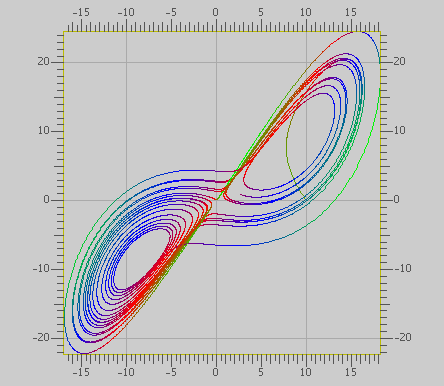
\includegraphics[width=1\textwidth]{lorenz-mx-plot.png}}
\end{column}
\end{columns}
\end{frame}

\begin{frame}[fragile]

\fontsize{7.8pt}{7.8pt}\selectfont\baselineskip=0pt
\begin{verbatim}
a = 10;     /* Parameters for the Lorenz Equations */
b = 8/3.0;
r = 28;

func Lorenz ( y, t ) = [ a*(y[1]-y[0]);  /* Matrix literal */
                        -y[0]*y[2] + r*y[0] - y[1];
                        y[0]*y[1] - b*y[2] ];

func RungeKutta( f, y, t, h ) {  /* Differential Equation Solver */
    k1 = h * f( y, t );              /* Invoke function f */
    k2 = h * f( y+0.5*k1, t+0.5*h );
    k3 = h * f( y+0.5*k2, t+0.5*h );
    k4 = h * f( y+k3, t+h );
    return y + (k1+k4)/6.0 + (k2+k3)/3.0;
}

N = 20000;
p = zeros(N+1,3);  /* matrix of zeros */
t = 0.0;
h = 0.001;
x = [ 10; 0; 10 ]; /* matrix literal */
p[0,:] = x';       /* matrix transpose */
 
for ( i = 1:N ) {
    x = RungeKutta( Lorenz, x, t, h );  /* Perform a step */
    p[i,:] = x';
    t += h;
}
 
colormap(3);
plot(p);     /* Plot points in the matrix */
return 0;    /* Terminate */
\end{verbatim}

\end{frame}

\begin{frame}[fragile]{YAPPL: Yet Another Probabilistic Programming Language}

{\small David Hu, Jonathan Huggins, Hans Hyttinen, Harley McGrew, 2011}

For programming statistical models: Church-inspired language

\begin{itemize}
\item  OCaml-like functional syntax with explicit types
\item \verb|fun| keyword for defining functions
\item Imperative code, too
\end{itemize}

Compiled to OCaml$^*$

$^*$This is no longer allowed; you must compile into LLVM

\end{frame}

\begin{frame}[fragile]

\fontsize{5.5pt}{5.5pt}\selectfont

\begin{verbatim}
###
  An implementation of the Dirichlet Process (DP) using memoization
###
fun float:beta float:a float:b = ~rand in 

# get a stick, breaking more if necessary 
fun int:pickastick (fun float int):sticks int:j =
    if ~rand < ~sticks j then j else ~pickastick sticks j+1
in

# generic Dirichlet process code
fun (fun int):DP float:alpha (fun int):proc =
    fun float:sticks int:x := ~beta 1.0 alpha in
    fun int:atoms  int:x := ~proc in
    fun int:f = ~atoms ~pickastick sticks 1 in
    f # return f
in

fun (fun (fun int) float):DPmem float:alpha (fun int float):proc =
    fun (fun int):dps float:arg := 
        fun int:apply = ~proc arg in
        ~DP alpha apply 
    in
    fun (fun int):dp float:arg = ~dps arg in
    dp
in

# this function will create Dirichlet process draws with geometric base distribution
let (fun (fun int) float):geom_dp = ~DPmem 1.0 geom in
 
# this is a DP draw with geometric base distribution with q = .2
let (fun int):mydraw = ~geom_dp .2 in

# use a tail-recursive loop to generate some samples from the Dirichlet Process
fun bool:loop int:i =
    ~print ~mydraw;
    if i > 0 then ~loop i - 1 else true
in
~seed;
~loop 30; ~print_line ~mydraw
\end{verbatim}

\end{frame}

\section{Graphics Languages: CAL, CLAM, curve}

\begin{frame}{CAL: Concise Animation Language}

Tianliang Sun,
Xinan Xu,
Jingyi Guo, 2013

\begin{itemize}
\item C-like syntax
\item User-defined functions
\item Structs
\item OpenGL calls
\end{itemize}
 
C-like language compiles into LLVM IR linked to OpenGL

\end{frame}

\begin{frame}[fragile]
\begin{columns}
\begin{column}{0.5\textwidth}
\fontsize{7pt}{7pt}\selectfont
\begin{verbatim}
int i = 0, j = 0, size = 10;

struct point_or_shape {
  point pt;
  shape shp;
};

int add_point_or_shape(int  x, int y,
            struct point_or_shape pos){
  if(x == y || x == size - y - 1)
    add_shape(pos.shp);
  else
    add_point(pos.pt);
  return 0;
}

int main(){
  struct point_or_shape pos;
  point pt;
  shape shp;

  for(i = 0; i < size; i=i++){
    for(j = 0; j < size; j=j++){
      pt.x=0.2*j+0.1-1.0;
      pt.y=-0.2*i-0.1+1.0;
      pt.vx=pt.y+pt.x;
      pt.vy=pt.x-pt.y;
      pt.r=pt.x/2.0+0.5;
      pt.g=pt.y/2.0+0.5;
      pt.b=0.0;
\end{verbatim}
\end{column}
\begin{column}{0.5\textwidth}
\fontsize{7pt}{7pt}\selectfont
\begin{verbatim}
      shp.size=0.2;
      shp.x=0.2*j+0.1-1.0;
      shp.y=-0.2*i-0.1+1.0;
      shp.vy=shp.x/2.0+shp.y;
      shp.vx=shp.y/2.0-shp.x;
      shp.r=shp.x/2.0+0.5;
      shp.g=shp.y/2.0+0.5;
      shp.b=1.0;
      shp.omega=1.0;
      pos.pt = pt;
      pos.shp = shp;
          wait(0.05);
      add_point_or_shape(j, i, pos);
    }
  }
  for(i=0;i<size*size;i=i++){
          wait(0.05);
        pop_shape();
        pop_point();
  }
 
  return 0;
}
\end{verbatim}
\end{column}
\end{columns}
\end{frame}

\begin{frame}{CLAM: Concise Linear Algebra Manipulation Language}

{\small Jeremy Andrus, Robert Martin, Kevin Sun, Yongxu Zhang, 2011}

Image-processing language

\begin{itemize}
\item Images with multiple channels (arrays, e.g., Red, Green)
\item Calculations: either literal C code or matrices
\item Kernel: sequence of calculations assembled with \texttt{\char`\|}
\item Convolution operator \texttt{**}
\end{itemize}

Compiles into C++ with extensive use of templates$^*$

$^*$This is no longer allowed; you must compile into LLVM

\end{frame}

\begin{frame}[fragile]

\fontsize{7.5pt}{7.5pt}\selectfont
\begin{verbatim}
Image srcimg = imgread(1);

/* Calc: functions on images */

/* # is "escape to C" */
Calc Lum := #[(3*Red + 6*Green + 1*Blue)/10]#;
Calc sobelG<Uint8>:=
   #[sqrt((float)sobelGx*sobelGx + (float)sobelGy*sobelGy)]#;
Calc sobelTheta<Angle>:= #[atan((float)sobelGy/(float)sobelGx)]#;

srcimg |= Lum; /* Calculate luminance of source image */

Calc sobelGx<Uint8> := [1 / 1]{ -1  0 +1 , /* Convolution kernel */
                                -2  0 +2 ,
                                -1  0 +1 };
Calc sobelGy<Uint8> := [1 / 1]{ +1 +2 +1 ,
                                 0  0  0 ,
                                -1 -2 -1 };

Kernel sobel = | @sobelGx | @sobelGy | sobelG; /* Build up kernel */
sobel |= sobelTheta; /* Add another kernel */

Image edges = srcimg:Lum ** sobel; /* Convolve with sobel */

Image output;
output:Red   = edges:sobelG; /* Output B&W */
output:Green = edges:sobelG;
output:Blue  = edges:sobelG;

imgwrite( output, "png", 2);
\end{verbatim}

\end{frame}

\begin{frame}{curve: Vector Graphics Animation}

{\small Kun An,
John Chan,
David Mauskop,
Wisdom Omuya,
Zitong Wang, 2012}

C-like language for animating vector graphics

\begin{itemize}
\item \texttt{int}, \texttt{Point}, \texttt{Curve}, and \texttt{Layer} types
\item Wrote their own standard library with functions like \texttt{rectangleXY}
\end{itemize}

Compiles into bytecode and interpreted

\end{frame}

\begin{frame}[fragile]
\fontsize{9pt}{10pt}\selectfont
\begin{verbatim}
int drawTree(int x, int y, int n) {
  Curve left;
  Curve right;

  if (n == 0) return 1;

  drawTree(x - exp(2, n), y - 50, n - 1);
  drawTree(x + exp(2, n), y - 50, n - 1);

  left = lineP((x, y), (x - exp(2, n), y - 50));
  right = lineP((x, y), (x + exp(2, n), y - 50));
  
  draw([left, right]);
  pause(100);
  return 1;
}
\end{verbatim}
\end{frame}

\begin{frame}
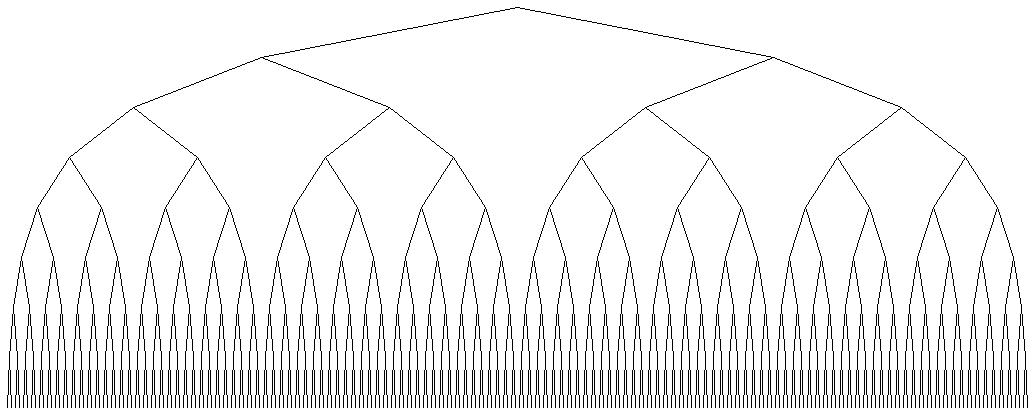
\includegraphics[width=\textwidth]{curve-language-tree.png}
\end{frame}

\section{C- and Java-Like Languages: Cpi, Dice}

\begin{frame}{Cpi: A C dialect for the Raspberry Pi}

{\small Edward Garcia, Niket Kandya,  
 Naveen Revanna, Sean Yeh, 2013}

Stripped-down C

\begin{itemize}
\item Integers, characters, pointers, arrays, structs
\item User-defined functions
\item for, if, case, while statements
\end{itemize}

Compiles into ARM V6 assembly

\end{frame}

\begin{frame}[fragile]
\begin{columns}
\begin{column}{0.5\textwidth}
\fontsize{7pt}{7pt}\selectfont
\begin{verbatim}
int checkrow(char board[], int row){
    int x1;
    int x2;
    x1 = row + 1;
    x2 = row + 2;
    if (board[row] == board[x1]){
        if (board[x1] == board[x2]){
            if (board[row] != ' '){
                printf("Row win!\n");
                return 1;
            }
        }
    }
    return 0;
}

int checkcol(char board[], int col){
    int x1;
    int x2;
    x1 = col + 3;
    x2 = col + 6;
    if (board[col] == board[x1]){
        if (board[x1] == board[x2]){
            if (board[col] != ' '){
                printf("Column win!\n");
                return 1;
            }
        }
    }
    return 0;
}
\end{verbatim}
\end{column}
\begin{column}{0.5\textwidth}
\fontsize{7pt}{7pt}\selectfont
\begin{verbatim}
int checkboard(char board[]){
    int result;
    int j;
    result = 0;

    for (j = 0; j < 3; j = j + 1){
        result = result +
                 checkrow(board, 3*j) +
                 checkcol(board, j);
    }

    // Check diags
    if (board[0] != ' '){
        if (board[0] == board[4]){
            if (board[4] == board[8]){
                result = 1;
            }
        }
    }
    if (board[2] != ' '){
        if (board[2] == board[4]){
            if (board[4] == board[6]){
                result = 1;
            }
        }
    }

    return result;
}
\end{verbatim}
\end{column}
\end{columns}
\end{frame}

\begin{frame}[fragile]
\begin{columns}
\begin{column}{0.4\textwidth}
\fontsize{7pt}{7pt}\selectfont
\begin{verbatim}
int printboard(char board[]){
    printf("|%c|%c|%c|\n", board[0],
           board[1],board[2]);
    printf("-------\n");
    printf("|%c|%c|%c|\n", board[3],
           board[4],board[5]);
    printf("-------\n");
    printf("|%c|%c|%c|\n", board[6],
           board[7],board[8]);
    return 0;
}

char getchar(int p){
    if (p == 1){
        return 'O';
    }
    return 'X';
}

int main()
{
    int player;
    int winner;
    int choice;
    int valid;
    int i;
    int count;
    char board[9];
    char tempc;
\end{verbatim}
\end{column}
\begin{column}{0.6\textwidth}
\fontsize{7pt}{7pt}\selectfont
\begin{verbatim}
    board[0] = ' ';    board[1] = ' ';
    board[2] = ' ';    board[3] = ' ';
    board[4] = ' ';    board[5] = ' ';
    board[6] = ' ';    board[7] = ' ';
    board[8] = ' ';    board[9] = ' ';

    printf("Player 1: 'O'\nPlayer 2: 'X'\n\n");
    printf("Valid inputs are 0-9\n\n");

    count = 0; winner = 0; player = 1;

    while (winner == 0){
        printboard(board);

        valid = 0;
        while(valid == 0){
            printf("Player %d, enter your move: ",
                   player);
            printf("\n");

            scanf("%d", &choice);

            valid = 1;
            if (choice < 0){ valid = 0; }
            if (choice > 9){ valid = 0; }
            if (valid == 1){ 
                if (board[choice] != ' '){
                    valid = 0;
                }
            }
        }
\end{verbatim}
\end{column}
\end{columns}

\end{frame}

\begin{frame}[fragile]
\begin{columns}
\begin{column}{0.5\textwidth}
\fontsize{7pt}{7pt}\selectfont
\begin{verbatim}
        tempc = getchar(player);
        board[choice] = tempc;
        if (checkboard(board) > 0){
            printboard(board);
            printf("Winner is Player %d!\n", player);
            winner = player;
        }

        if (player == 1) {
           player = 2;
        } else {
           player = 1;
        }

        count = count + 1;
        if (count >= 9){
            if (winner == 0){
                printf("No one wins!\n");
                winner = -1;
            }
        }
    }
    return 0;
}
\end{verbatim}
\end{column}
\end{columns}
\end{frame}

\begin{frame}{Dice: ``Java, but worse''}

{\small David Watkins, Emily Chen, Philip Schiffrin, Khaled Atef, 2015}

Simplified Java language

\begin{itemize}
\item Classes, inheritance
\item Methods, virtual function dispatch
\item Arrays
\item Strings
\item File I/O
\end{itemize}

Compiles to LLVM

\end{frame}

\begin{frame}[fragile]
\fontsize{6pt}{6pt}\selectfont
\begin{verbatim}
include("stdlib");

class Player {
    public class LocationObj placeTile(bool retry)   {
        return new LocationObj();
    }

    public void setResult(class LocationObj move) { 
    }
}

class HumanPlayer extends Player {
    private class Board board;
    public int myPieceType;

    constructor()   {
        this.board = new Board();
        this.myPieceType = 2;
        class Board b = this.board;
        b.initializeBoard();
    }

    public class LocationObj placeTile(bool retry)   {
        if (this.myPieceType == 2)
            this.myPieceType = 1;
        if (retry){
            print("Last move was invalid. Retry.\n"); }
        print("It's your turn\n");
        class Board b = this.board;
        b.printBoard();

        print("Please enter your move\n");
        class LocationObj move = this.getLocationObjChoice();
        int temp = this.myPieceType;
        b.setPlayerMove(move, temp);
        return move;
    }
\end{verbatim}
\end{frame}

\begin{frame}[fragile]
\fontsize{4.8pt}{4.8pt}\selectfont
\begin{verbatim}
   public void setResult(class LocationObj move) {
        int temp = this.myPieceType;
        if (temp == 1) {
            bool one = (move.getHorizontal() == 3);
            bool two = (move.getHorizontal() == 4);
            bool three = (move.getVertical() == 3);
            bool four = (move.getVertical() == 4);
            bool five = ((one or two ) and (three or four)); 
             if(not five){
                this.myPieceType = 0;
                }
        }
        int opponentPieceType;
        int temp2 = this.myPieceType;
        if (temp2 == 0){
            opponentPieceType = 1; }
        else {
            opponentPieceType = 0;}

        class Board b = this.board;
        b.setPlayerMove(move, opponentPieceType);
    }

    private class LocationObj getLocationObjChoice(){ 
        char[] userInput;
        class String uInput;
        class Board b = new Board();
        class LocationObj move = null;
        int temp = this.myPieceType;    
        while (not (b.isValid(move, temp))) { 
            print("You are " , this.myPieceType , ". What is the x location of your next move?");
            userInput = input();
            uInput = new String(userInput);
            int x = uInput.toInteger();
            print("You are " , this.myPieceType , ". What is the y location of your next move?");
            userInput = input();
            uInput = new String(userInput);
            int y = uInput.toInteger();
            move = new LocationObj(x - 1, y - 1);
            bool one = b.isValid(move,temp);
            if (not one){
                print("invalid move, try again.\n"); }
        } 
        return move;
    }
}
\end{verbatim}
\end{frame}

\section{Hardware Description Languages: EHDL}

\begin{frame}{EHDL: Hardware Description Language}

{\small  
Paolo Mantovani,
Mashooq Muhaimen,
Neil Deshpande,
Kaushik Kaul,
2011
}

\begin{itemize}
\item Bit vectors/binary numbers of a specific width
\item User-defined functions
\item If-then-else, switch-case
\item \texttt{POS} denotes clock boundaries in imperative code
\item \texttt{while} loops have an implicit clock
\item Arrays for little memories
\end{itemize}

Compiles into VHDL$^*$

$^*$This is one of the few possible exceptions to the LLVM backend
rule.  You need to convince me that a non-LLVM-backend is the best
choice for your project.

\end{frame}

\begin{frame}[fragile]
\fontsize{7pt}{7pt}\selectfont
\begin{verbatim}
(int(1) sum, int(1) carry) fulladder(int(1) a, int(1) b, int(1) carryin){        
        sum = a ^ b ^ carryin;
        carry = (a && b) ^ (carryin && (a ^ b));       
}

(int(4) s, int(1) overflow) main(int(4) a, int(4) b, int(1) carryin) {         
        int(1) sum[4];
        int(1) carry[4];

        (sum[0], carry[0]) = fulladder(a(0),b(0),carryin);
        (sum[1], carry[1]) = fulladder(a(1),b(1),carry[0]);
        POS(1);
        (sum[2], carry[2]) = fulladder(a(2),b(2),carry[1]);
        (sum[3], carry[3]) = fulladder(a(3),b(3),carry[2]);
        POS(1);

        s(3) = sum[3]; s(2) = sum[2];
        s(1) = sum[1]; s(0) = sum[0];

        if ((a>0) && (b>0) && (sum[3]<0) )overflow = 1;
        else if ((a<0) && (b<0) && (sum[3]>0) )overflow = 1;
        else overflow = 0;
}
\end{verbatim}

\centerline{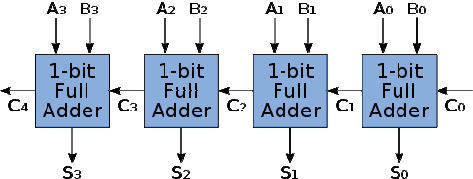
\includegraphics[width=0.5\textwidth]{ehdl-ripple-carry-adder.pdf}}
\end{frame}

\begin{frame}[fragile]
\fontsize{8pt}{8pt}\selectfont
\begin{verbatim}
/* Sieve of Eratosthenes */

/* emits all the prime numbers less than m. m must be less than 200
as there is a bounded buffer of size 200 that is being used */
(int(32) primes=2) main (int(32) m) { 
        
        int(1) a[200]; 
        int(1) sig; 
        int(32) n = 2;
        int(32) k = 2;
         
        while (n <= m) {
              
            if ((a[n] == 0) && (k <= m))  {
                 if (k == n) {   
                      primes = n; /* generate output */
                 } else { 
                   a[k] = 1; 
                 } 
                 k = k + n;    
            }else {
                 n = n + 1;
                 k = n + 1;                   
            }         
        }             /* Implicit clock cycle here */
}
\end{verbatim}
\end{frame}

\section{Music Languages: Note-Hashtag}

\begin{frame}{Note-Hashtag: Music Synthesis Language}

Kevin Chen, Brian Kim, Edward Li, 2015

\begin{itemize}
\item Vectors of notes with durations
\item Functional-like transformations (e.g., scale up two pitches)
\item Rhythm can be projected on a melody
\item Melody can be projected onto a key signature
\item User-defined composite types
\end{itemize}

Generates C++ code that produces a .WAV file$^*$

$^*$Now, would have to compile into LLVM that, when run, produces a .WAV file

\end{frame}

\begin{frame}[fragile]
\fontsize{7.5pt}{7.5pt}\selectfont
\begin{verbatim}
// Twinkle, Twinkle Little Star
// main parts
intro = quarter:[ 1 1 5 5 6 6 ] . half:5
chorus = Rhythms intro : [ 4 4 3 3 2 2 1 ]
bridge = Relative 1 chorus

// the tune
twinkle_melody = intro . chorus . bridge . bridge . intro . chorus
twinkle_harmony = Relative 2 twinkle_melody

// supporting line
base = eighth:[ 1 5 3 5 ]
rise = eighth:[ 1 6 4 6 ]
fall = eighth:[ 7@(-1)  5 2 5 ]
bottom = eighth:[ 6@(-1)  5 1 5 ]

intro_accomp = base . base . rise . base
chorus_accomp = fall . base . bottom . base
bridge_accomp = base . fall . base . fall

// the accompaniment
accomp = intro_accomp . chorus_accomp . bridge_accomp . \
            bridge_accomp . intro_accomp . chorus_accomp
twinkle_bass = Octave (-1) accomp

// the song
twinkle = Parallel { twinkle_melody twinkle_harmony twinkle_bass }
twinkle$volumes = { 1.0 0.5 0.5 }
Render twinkle "twinkle.wav"
\end{verbatim}
\end{frame}

\begin{frame}[fragile]
\fontsize{8pt}{8pt}\selectfont
\begin{verbatim}
tempo = 74

// stairway to heaven - led zeppelin
intro = eighth : [ 6@(-1)  1 3 6  7,5#  3 1 7 ] .\
  e : [ 1@1,5  3 1  1@1  4#,4#@(-1)  2  6@(-1)  4 ] .\
  e : [ 3,4@(-1)  1  6@(-1) ] . q:1 . e : [ 3 1  6@(-1) ]
fin_chord = 5@(-1),7@(-1)
fin = e:fin_chord,7@(-2) . Relative 1 ([ e (q+e) ]:fin_chord,5@(-2))
intro = intro . fin . Octave (-1) (e:[ 6@(-1) 4 3 ])

// note that the next phrase is the same except for the first and last notes
intro_next = EndWith ([ e e h ]:Chords fin . q:~) (StartWith (e:6@(-2)) intro)

stairway = intro . intro_next

all_the_way_to_heaven = Parallel { stairway }
Render all_the_way_to_heaven "stairway_to_heaven.wav"
\end{verbatim}
\end{frame}

\end{document}
